\documentclass[12pt, twoside]{article}
\usepackage[francais]{babel}
\usepackage[T1]{fontenc}
\usepackage[latin1]{inputenc}
\usepackage[left=7mm, right=7mm, top=5mm, bottom=5mm]{geometry}
\usepackage{float}
\usepackage{graphicx}
\usepackage{array}
\usepackage{multirow}
\usepackage{amsmath,amssymb,mathrsfs}
\usepackage{soul}
\pagestyle{empty}
\begin{document}


\section*{\center{Aide individualis�e: Signe de ax+b}}

\subsection*{Faire un tableau de signes}

\begin{enumerate}
  \item Compl�ter le tableau:
  
 \begin{center}
  $
  \begin{array}{|c|m{8mm}|m{8mm}|m{8mm}|m{8mm}|m{8mm}|m{8mm}|m{8mm}|m{8mm}|m{8mm}|} 
   \hline
   x & -2 & -1 & 0 \ & 1\ & 2 \ & 3 \ & 4 \ & 5 \ & 6\  \\
  \hline
  5x-10 & -20 & \ & \ &\  &\  & \ &\  &\  &\\ 
  \hline
  \end{array}
$
\end{center}
\item Pour quelle valeur de $x$, $5x-10$ vaut 0?
\item Donner deux exemples de valeurs de $x$ pour lesquelles $5x-10$ est
n�gatif?
\item Donner deux exemples de valeurs de $x$ pour lesquelles $5x-10$ est
positif?

\medskip

D'apr�s les valeurs trouv�es, il \ul{semblerait} que $5x-10$ soit n�gatif pour
$x \ldots \ldots \ldots$, nul pour $x=\ldots$ et positif pour $x \ldots \ldots
\ldots$.

V�rifions-le par le calcul:
\item R�soudre:
$5x-10=0$

$5x-10<0$

$5x-10>0$

\item Compl�ter:

 Pour $x \in ]- \infty; \ldots [$, $5x-10$ est n�gatif.
 
Pour $x=\ldots$, $5x-10$ est nul.

 Pour $x \in ]2;+ \infty[$, $5x-10$ est \ldots \ldots \ldots \ldots \ldots.
 
 \enskip
 Sch�matisons les trois derni�res phrases dans un tableau:   
 \begin{center}
 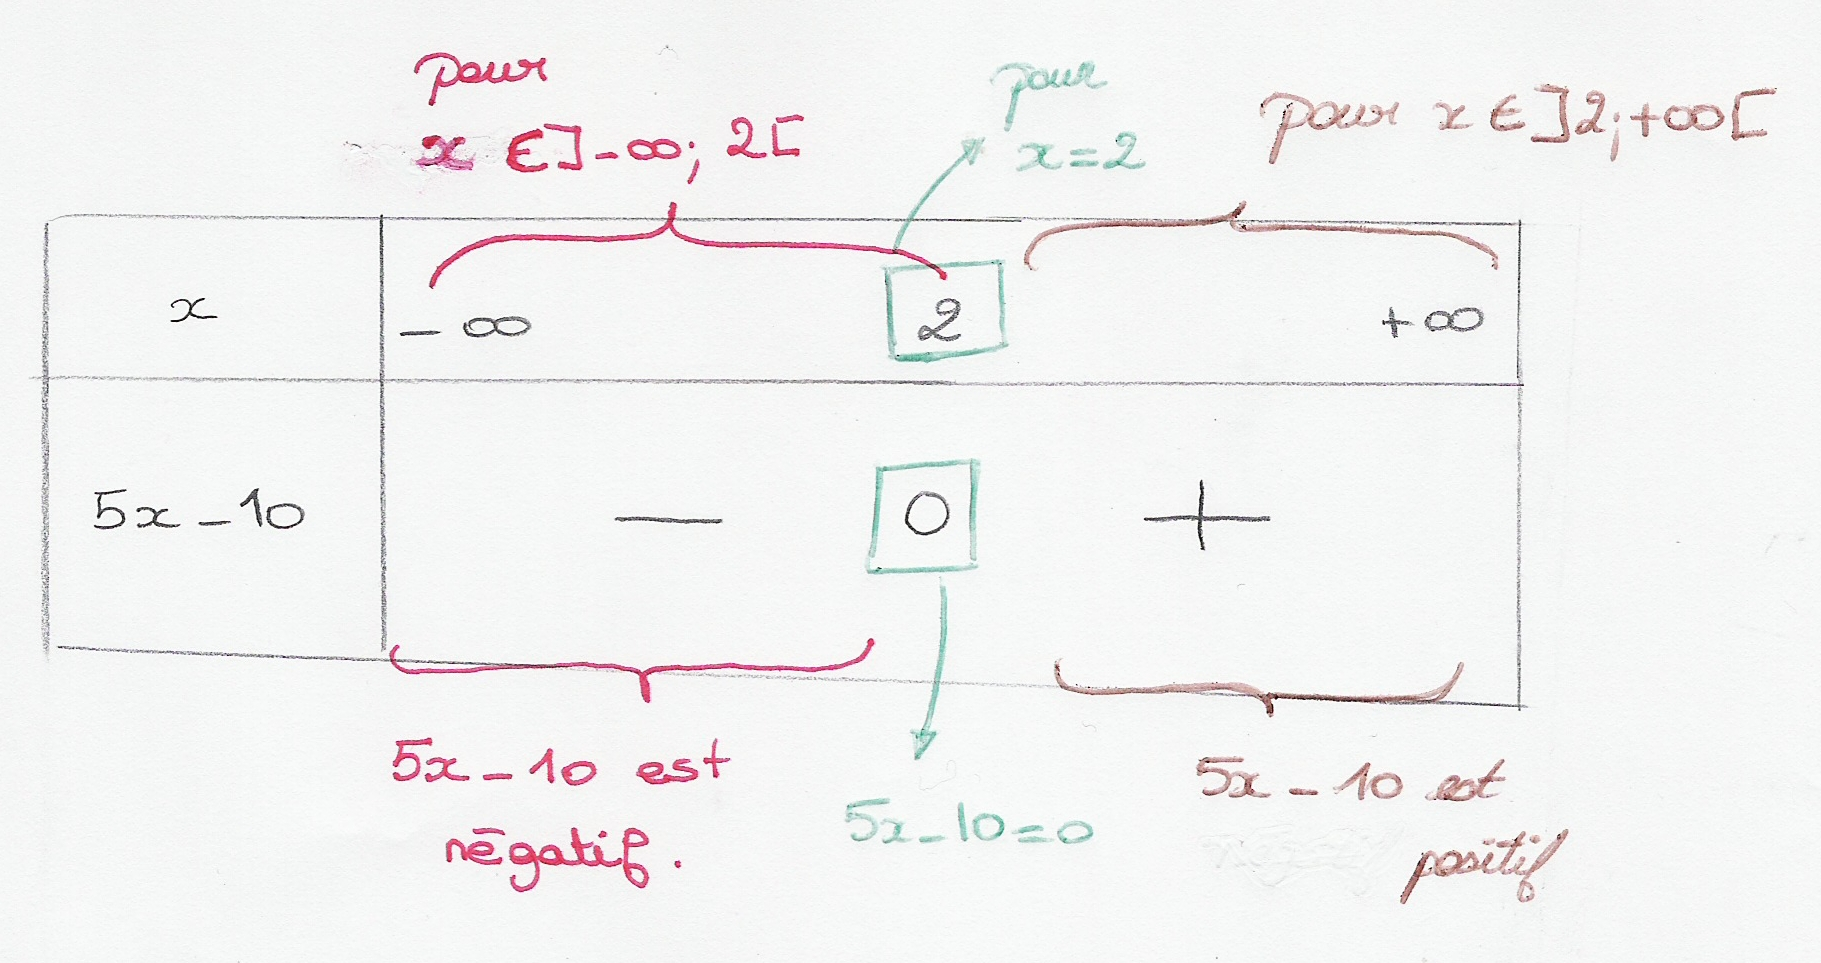
\includegraphics[width=14cm]{images/ex.jpg}
 \end{center}       
\end{enumerate}
 
\subsection*{Lire un tableau de signes}

\begin{center}

$\begin{array}{|c|ccccc|}
\hline
 x & -\infty & \ \ \ \ \ \ \ \ \ \ \ & 1 &\ \ \ \ \  \ \ \ \ \ & +\infty \\
 \hline
 1-x & \ \ & + & \ \ \ \ 0 \ \ \ \ & - & \ \ \\
 \hline
 \end{array}$
\end{center}

\begin{enumerate}
  \item Pour quelle valeur de $x$, $1-x$ vaut $0$?
  \item Donner des exemples de valeurs de $x$ pour lesquelles $1-x$ est n�gatif.
  \item Pour quelle valeur de $x$, $1-x$ est-il positif? (donner la r�ponse sous
  forme d'intervalle)
  \item Pour $x=-2$, quel est le signe de $1-x$? M�me question pour $x=4$.
\end{enumerate}

\subsection*{A vous de jouer\ldots}

\begin{enumerate}
  \item Faire le tableau de signes de $7x+3$.
  
  \textbf{M�thode:} 
  \begin{itemize}
    \item [$\bullet$] R�soudre $7x+3=0$.
    \item [$\bullet$] R�soudre $7x+3<0$.
    \item [$\bullet$] Compl�ter le tableau de signes.
  \end{itemize}
  
  \item Faire le tableau de signes de $-4x+5$.
  \item R�soudre $(2x-1)(x+6)<0$.
  
  \textbf{M�thode:}
  \begin{itemize}
    \item [$\bullet$] R�soudre $2x-1=0$.
    \item [$\bullet$] R�soudre $x+6=0$.
    \item [$\bullet$] Mettre les valeurs trouv�es dans le tableau (dans la
    ligne ``des $x$'')
    \item [$\bullet$] Etudier le signe de $2x-1$ sur chaque intervalle et
    compl�ter le tableau.
    \item [$\bullet$] Etudier le signe de $x+6$ sur chaque intervalle et
    compl�ter le tableau (juste en dessous).
    \item [$\bullet$] Etudier le signe du produit en utilisant la r�gle des
    signes, puis lire le tableau pour conclure.
  \end{itemize}
\end{enumerate}


\end{document}
